\documentclass[11pt, letterpaper]{article}

% Fonts and Encoding
\usepackage[utf8]{inputenc}
\usepackage[T1]{fontenc}
\usepackage{lmodern} % High-quality Latin Modern vector font

% Math and Symbols
\usepackage{amsmath, amssymb, amsthm, amsfonts, mathrsfs, mathtools}

% Layout and Geometry
\usepackage{geometry}
\geometry{letterpaper, margin=1in}
\setlength{\parindent}{0pt}
\setlength{\parskip}{0.6em}

% Formatting and Graphics
\usepackage{graphicx, xcolor, enumitem, booktabs, array, tabularx}

% TikZ for Illustrations
\usepackage{tikz}
\usetikzlibrary{arrows.meta, positioning, shapes.geometric, calc, backgrounds, matrix}

% Clickable Links and TOC
\usepackage{hyperref}
\hypersetup{
    colorlinks=true,
    linkcolor=blue,
    filecolor=magenta,      
    urlcolor=cyan,
    pdftitle={Advanced Mathematics Topic},
}

% Theorem Environments
\newtheorem{theorem}{Theorem}[section]
\newtheorem{lemma}[theorem]{Lemma}
\newtheorem{proposition}[theorem]{Proposition}
\newtheorem{corollary}[theorem]{Corollary}
\theoremstyle{definition}
\newtheorem{definition}{Definition}[section]
\newtheorem{axiom}{Axiom}[section]
\newtheorem{example}{Example}[section]
\theoremstyle{remark}
\newtheorem{remark}{Remark}[section]

% Custom Commands (Enforced standard notation)
\newcommand{\R}{\mathbb{R}}
\newcommand{\N}{\mathbb{N}}
\newcommand{\Z}{\mathbb{Z}}
\newcommand{\Q}{\mathbb{Q}}
\newcommand{\E}{\mathbb{E}}
\newcommand{\Prob}{\mathbb{P}}
\newcommand{\F}{\mathcal{F}}

\begin{document}

\title{Advanced Abstract Mathematics: Injective, Surjective, and Bijective Functions \\ \Large Comprehensive Practice Problem Set}
\author{Tashfeen Omran}
\date{November 12, 2026}

\maketitle
\tableofcontents
\newpage

\section{Concept Checklist \& Question Mapping}

The following table outlines the core theoretical concepts, logical structures, and proof techniques extracted from the foundational text. Each concept is mapped to specific problems in the problem set to ensure comprehensive coverage.

\renewcommand{\arraystretch}{1.5}
\begin{tabularx}{\textwidth}{l X >{$\displaystyle}c<{$}}
\toprule
\textbf{ID} & \textbf{Concept / Technique} & \text{\textbf{Mapped Problems}} \\
\midrule
C1 & Algebraic Verification of Injectivity (Direct Proof) & 1, 2, 3, 5, 28 \\
C2 & Algebraic Verification of Surjectivity (Direct Proof) & 1, 3, 4, 5, 27 \\
C3 & Counterexample Generation (Falsifying Injectivity) & 4, 6, 7, 9, 10, 23 \\
C4 & Counterexample Generation (Falsifying Surjectivity) & 2, 6, 7, 8, 10 \\
C5 & Abstract Set-Theoretic Proofs (Element-Chasing) & 11, 12, 13, 14, 15 \\
C6 & Function Composition Properties ($g \circ f$) & 16, 17, 18, 19, 20 \\
C7 & Pigeonhole Principle \& Cardinality Arguments & 8, 9, 24, 25, 26 \\
C8 & Relations vs. Functions (Well-definedness) & 21 \\
C9 & Modular Arithmetic in Relations \& Functions & 22, 23 \\
C10 & Real-World Modeling (CDFs, Inverse Transform, ML) & 27, 28 \\
C11 & Identifying Logical Flaws in Proofs & 29, 30 \\
\bottomrule
\end{tabularx}

\newpage

\section{Problem Set}

\textbf{Algebraic Verification \& Counterexamples}

\begin{enumerate}[label=\textbf{\arabic*.}]
    \item Prove that the function $f : \R \to \R$ defined by $f(x) = 3x - 7$ is bijective.
    \item Let $f : \Z \to \Z$ be defined by $f(n) = 4n + 3$. Prove that $f$ is injective but not surjective.
    \item Let $f : \R \setminus \{2\} \to \R \setminus \{5\}$ be defined by $f(x) = \frac{5x+1}{x-2}$. Prove that $f$ is bijective.
    \item Let $f : \Z \times \Z \to \Z$ be defined by $f(m,n) = m + n$. Prove that $f$ is surjective but not injective.
    \item Prove that the function $f : \R \to \R$ defined by $f(x) = x^3 - 3x^2 + 3x - 1$ is bijective.
    \item Let $f : \R \to \R$ be defined by $f(x) = |x-3| + 2$. Find counterexamples to show that $f$ is neither injective nor surjective.
    \item Let $f : \Z \to \Z$ be defined by $f(n) = n^2 + n$. Prove that $f$ is neither injective nor surjective.
    \item Is there a function $f : \N \to \N$ that is surjective but not injective? If so, construct one. (Assume $\N = \{1, 2, 3, \dots\}$).
    \item Is there a function $f : \N \to \N$ that is injective but not surjective? If so, construct one.
    \item Let $f : \R \to \R$ be defined by $f(x) = e^{x^2}$. Prove that $f$ is neither injective nor surjective.
\end{enumerate}

\textbf{Abstract Set-Theoretic Proofs}

\begin{enumerate}[label=\textbf{\arabic*.}, resume]
    \item Let $f : X \to Y$ be a function, and let $A, B \subseteq X$. Prove that $f(A \cup B) = f(A) \cup f(B)$.
    \item Let $f : X \to Y$ be a function, and let $C, D \subseteq Y$. Prove that $f^{-1}(C \cap D) = f^{-1}(C) \cap f^{-1}(D)$.
    \item Let $f : X \to Y$ be a function. Prove that if $f$ is injective, then $f(A \cap B) = f(A) \cap f(B)$ for all $A, B \subseteq X$.
    \item Let $f : X \to Y$ be a function. Prove that $f$ is surjective if and only if $f(f^{-1}(B)) = B$ for all $B \subseteq Y$.
    \item Let $f : X \to Y$ be a function. Prove that if $f$ is injective, then $f^{-1}(f(A)) = A$ for all $A \subseteq X$.
\end{enumerate}

\textbf{Function Composition}

\begin{enumerate}[label=\textbf{\arabic*.}, resume]
    \item Let $f : A \to B$ and $g : B \to C$ be functions. Prove that if $g \circ f$ is surjective, then $g$ is surjective.
    \item Let $f : A \to B$ and $g : B \to C$ be functions. Prove that if $g \circ f$ is injective and $f$ is surjective, then $g$ is injective.
    \item Let $f : A \to B$ and $g : B \to C$ be functions. Find a counterexample where $g \circ f$ is bijective, but $g$ is not injective.
    \item Let $f : A \to B$ and $g : B \to C$ be functions. Find a counterexample where $g \circ f$ is bijective, but $f$ is not surjective.
    \item Prove that a function $f : A \to B$ is bijective if and only if there exists a function $g : B \to A$ such that $g \circ f = \text{id}_A$ and $f \circ g = \text{id}_B$, where $\text{id}_X$ denotes the identity function on set $X$.
\end{enumerate}

\textbf{Relations, Modular Arithmetic, and Cardinality}

\begin{enumerate}[label=\textbf{\arabic*.}, resume]
    \item Let $A = \{1, 2, 3, 4\}$ and $B = \{2, 4, 6, 8\}$. A relation $R$ from $A$ to $B$ is defined by $aRb$ if $a \mid b$ and the integer $b/a$ is odd. Is $R$ a valid function from $A$ to $B$? Justify your answer.
    \item Let $f : \Z_5 \to \Z_5$ be defined by $f(x) \equiv (3x + 2) \pmod 5$. Prove that $f$ is bijective.
    \item Let $f : \Z_6 \to \Z_6$ be defined by $f(x) \equiv (2x + 1) \pmod 6$. Is $f$ injective? Prove or disprove.
    \item Let $A$ and $B$ be finite sets such that $|A| = |B|$. Prove that a function $f : A \to B$ is injective if and only if it is surjective.
    \item Let $A$ be a set with 5 elements and $B$ be a set with 4 elements. Prove rigorously using the Pigeonhole Principle that no function $f : A \to B$ can be injective.
    \item Prove that for any set $A$, there is no surjective function $f : A \to \mathcal{P}(A)$, where $\mathcal{P}(A)$ is the power set of $A$. (Cantor's Theorem).
\end{enumerate}

\textbf{Real-World Modeling \& Flawed Proofs}

\begin{enumerate}[label=\textbf{\arabic*.}, resume]
    \item \textbf{Quantitative Finance (Inverse Transform Sampling):} Let $F(x) = 1 - e^{-\lambda x}$ for $x \ge 0$ and $\lambda > 0$ (the Cumulative Distribution Function of an Exponential random variable). Prove that $F : [0, \infty) \to [0, 1)$ is a bijection. Then, derive the inverse function $F^{-1}(U)$ used to simulate this variable from a uniform random variable $U \in [0, 1)$.
    \item \textbf{Machine Learning (Normalizing Flows):} In generative modeling, transformations must be bijective. Let $f : \R \to \R$ be defined by $f(x) = x + \sigma(x)$, where $\sigma(x) = \frac{1}{1+e^{-x}}$ is the sigmoid function. Prove that $f$ is injective by analyzing its derivative.
    \item \textbf{Find the Flaw:} Identify the logical error in the following proof. \\
    \textit{Problem:} Prove that $f : \R \to \R$ defined by $f(x) = x^2$ is surjective. \\
    \textit{Flawed Proof:} Let $y \in \R$. We must find an $x \in \R$ such that $f(x) = y$. We set $x = \sqrt{y}$. Then $f(x) = (\sqrt{y})^2 = y$. Since we found an $x$ for every $y$, $f$ is surjective. $\blacksquare$
    \item \textbf{Find the Flaw:} Identify the logical error in the following proof. \\
    \textit{Problem:} Let $f : A \to B$ and $g : B \to C$. Prove that if $g$ is injective, then $g \circ f$ is injective. \\
    \textit{Flawed Proof:} Assume $g$ is injective. Let $a_1, a_2 \in A$ and assume $(g \circ f)(a_1) = (g \circ f)(a_2)$. This means $g(f(a_1)) = g(f(a_2))$. Because $g$ is injective, this implies $f(a_1) = f(a_2)$. Therefore, $a_1 = a_2$. Thus, $g \circ f$ is injective. $\blacksquare$
\end{enumerate}

\newpage

\section{Detailed Solutions}

\begin{proof}[Solution to Problem 1]
\textbf{Injectivity:} Let $a, b \in \R$ and assume $f(a) = f(b)$. Then $3a - 7 = 3b - 7$. Adding 7 to both sides yields $3a = 3b$. Dividing by 3 yields $a = b$. Thus, $f$ is injective. \\
\textbf{Surjectivity:} Let $y \in \R$. We must find an $x \in \R$ such that $f(x) = y$. Set $3x - 7 = y$. Solving for $x$, we get $x = \frac{y + 7}{3}$. Since $y \in \R$, $x \in \R$. Evaluating $f$ at this $x$ gives $f\left(\frac{y + 7}{3}\right) = 3\left(\frac{y + 7}{3}\right) - 7 = y + 7 - 7 = y$. Thus, $f$ is surjective. \\
Since $f$ is both injective and surjective, it is bijective.
\end{proof}

\begin{proof}[Solution to Problem 2]
\textbf{Injectivity:} Let $a, b \in \Z$ and assume $f(a) = f(b)$. Then $4a + 3 = 4b + 3 \implies 4a = 4b \implies a = b$. Thus, $f$ is injective. \\
\textbf{Non-Surjectivity:} Let $y = 0 \in \Z$. We seek an $n \in \Z$ such that $4n + 3 = 0$. Solving for $n$ yields $n = -\frac{3}{4}$. Since $-\frac{3}{4} \notin \Z$, there is no integer $n$ that maps to 0. Thus, $f$ is not surjective.
\end{proof}

\begin{proof}[Solution to Problem 3]
\textbf{Injectivity:} Let $a, b \in \R \setminus \{2\}$ and assume $f(a) = f(b)$. 
\[ \frac{5a+1}{a-2} = \frac{5b+1}{b-2} \]
Cross-multiplying yields:
\[ (5a+1)(b-2) = (5b+1)(a-2) \]
\[ 5ab - 10a + b - 2 = 5ab - 10b + a - 2 \]
Subtracting $5ab - 2$ from both sides:
\[ -10a + b = -10b + a \implies 11b = 11a \implies a = b \]
Thus, $f$ is injective. \\
\textbf{Surjectivity:} Let $y \in \R \setminus \{5\}$. We set $f(x) = y$ and solve for $x$:
\[ \frac{5x+1}{x-2} = y \implies 5x + 1 = y(x - 2) \implies 5x + 1 = yx - 2y \]
\[ 5x - yx = -2y - 1 \implies x(5 - y) = -2y - 1 \implies x = \frac{2y + 1}{y - 5} \]
Since $y \neq 5$, $x$ is a well-defined real number. We must ensure $x \neq 2$. If $x = 2$, then $2 = \frac{2y+1}{y-5} \implies 2y - 10 = 2y + 1 \implies -10 = 1$, a contradiction. Thus $x \in \R \setminus \{2\}$. Therefore, $f$ is surjective. \\
Since $f$ is injective and surjective, it is bijective.
\end{proof}

\begin{proof}[Solution to Problem 4]
\textbf{Surjectivity:} Let $y \in \Z$. We must find a pair $(m,n) \in \Z \times \Z$ such that $f(m,n) = y$. Let $m = y$ and $n = 0$. Both are integers. $f(y, 0) = y + 0 = y$. Thus, $f$ is surjective. \\
\textbf{Non-Injectivity:} Consider the distinct pairs $(1, 2)$ and $(2, 1)$ in $\Z \times \Z$. $f(1, 2) = 1 + 2 = 3$, and $f(2, 1) = 2 + 1 = 3$. Since $f(1, 2) = f(2, 1)$ but $(1, 2) \neq (2, 1)$, $f$ is not injective.
\end{proof}

\begin{proof}[Solution to Problem 5]
Notice that $f(x) = x^3 - 3x^2 + 3x - 1 = (x - 1)^3$. \\
\textbf{Injectivity:} Let $a, b \in \R$ and assume $f(a) = f(b)$. Then $(a - 1)^3 = (b - 1)^3$. Taking the real cube root of both sides (which is a well-defined, one-to-one operation on $\R$), we get $a - 1 = b - 1 \implies a = b$. Thus, $f$ is injective. \\
\textbf{Surjectivity:} Let $y \in \R$. Set $(x - 1)^3 = y$. Solving for $x$ yields $x = \sqrt[3]{y} + 1$. Since every real number has a unique real cube root, $x \in \R$. Evaluating $f$ gives $f(\sqrt[3]{y} + 1) = (\sqrt[3]{y} + 1 - 1)^3 = (\sqrt[3]{y})^3 = y$. Thus, $f$ is surjective. \\
Therefore, $f$ is bijective.
\end{proof}

\begin{proof}[Solution to Problem 6]
\textbf{Non-Injectivity:} We look for two distinct inputs that yield the same output. Let $x = 2$ and $x = 4$. 
\[ f(2) = |2 - 3| + 2 = |-1| + 2 = 3 \]
\[ f(4) = |4 - 3| + 2 = |1| + 2 = 3 \]
Since $f(2) = f(4)$ but $2 \neq 4$, $f$ is not injective. \\
\textbf{Non-Surjectivity:} The absolute value function is non-negative, so $|x - 3| \ge 0$ for all $x \in \R$. Thus, $f(x) = |x - 3| + 2 \ge 2$. Let $y = 0 \in \R$. There is no $x \in \R$ such that $f(x) = 0$, because $0 \not\ge 2$. Thus, $f$ is not surjective.
\end{proof}

\begin{proof}[Solution to Problem 7]
\textbf{Non-Injectivity:} Let $n = 0$ and $n = -1$. 
\[ f(0) = 0^2 + 0 = 0 \]
\[ f(-1) = (-1)^2 + (-1) = 1 - 1 = 0 \]
Since $f(0) = f(-1)$ but $0 \neq -1$, $f$ is not injective. \\
\textbf{Non-Surjectivity:} Let $y = -1 \in \Z$. We set $n^2 + n = -1 \implies n^2 + n + 1 = 0$. The discriminant of this quadratic is $1^2 - 4(1)(1) = -3 < 0$. Thus, there are no real solutions, and consequently no integer solutions. Since $-1$ has no pre-image, $f$ is not surjective.
\end{proof}

\begin{proof}[Solution to Problem 8]
Yes. Define $f : \N \to \N$ by $f(1) = 1$, and $f(n) = n - 1$ for $n \ge 2$. \\
\textbf{Surjectivity:} Let $y \in \N$. Then $y + 1 \in \N$ and $y + 1 \ge 2$. By definition, $f(y + 1) = (y + 1) - 1 = y$. Thus, every $y \in \N$ has a pre-image, so $f$ is surjective. \\
\textbf{Non-Injectivity:} Observe that $f(1) = 1$ and $f(2) = 2 - 1 = 1$. Since $f(1) = f(2)$ but $1 \neq 2$, $f$ is not injective.
\end{proof}

\begin{proof}[Solution to Problem 9]
Yes. Define $f : \N \to \N$ by $f(n) = n + 1$. \\
\textbf{Injectivity:} Let $a, b \in \N$ and assume $f(a) = f(b)$. Then $a + 1 = b + 1 \implies a = b$. Thus, $f$ is injective. \\
\textbf{Non-Surjectivity:} Let $y = 1 \in \N$. We set $n + 1 = 1 \implies n = 0$. However, $0 \notin \N$. Thus, 1 has no pre-image in $\N$, so $f$ is not surjective.
\end{proof}

\begin{proof}[Solution to Problem 10]
\textbf{Non-Injectivity:} Let $x = 1$ and $x = -1$. $f(1) = e^{1^2} = e$. $f(-1) = e^{(-1)^2} = e$. Since $f(1) = f(-1)$ but $1 \neq -1$, $f$ is not injective. \\
\textbf{Non-Surjectivity:} The exponential function $e^z > 0$ for all $z \in \R$. Let $y = -1 \in \R$. There is no $x \in \R$ such that $e^{x^2} = -1$. Thus, $f$ is not surjective.
\end{proof}

\begin{proof}[Solution to Problem 11]
We prove mutual subset inclusion. \\
\textbf{Part 1: $f(A \cup B) \subseteq f(A) \cup f(B)$.} Let $y \in f(A \cup B)$. By definition, there exists $x \in A \cup B$ such that $f(x) = y$. Since $x \in A \cup B$, either $x \in A$ or $x \in B$. If $x \in A$, then $f(x) \in f(A)$, so $y \in f(A)$. If $x \in B$, then $f(x) \in f(B)$, so $y \in f(B)$. In either case, $y \in f(A) \cup f(B)$. \\
\textbf{Part 2: $f(A) \cup f(B) \subseteq f(A \cup B)$.} Let $y \in f(A) \cup f(B)$. Then $y \in f(A)$ or $y \in f(B)$. If $y \in f(A)$, there exists $x \in A$ such that $f(x) = y$. Since $x \in A$, $x \in A \cup B$, so $f(x) \in f(A \cup B)$. The same logic applies if $y \in f(B)$. Thus, $y \in f(A \cup B)$. \\
Therefore, $f(A \cup B) = f(A) \cup f(B)$.
\end{proof}

\begin{proof}[Solution to Problem 12]
We prove mutual subset inclusion. \\
\textbf{Part 1: $f^{-1}(C \cap D) \subseteq f^{-1}(C) \cap f^{-1}(D)$.} Let $x \in f^{-1}(C \cap D)$. By definition of the pre-image, $f(x) \in C \cap D$. This means $f(x) \in C$ and $f(x) \in D$. Since $f(x) \in C$, $x \in f^{-1}(C)$. Since $f(x) \in D$, $x \in f^{-1}(D)$. Therefore, $x \in f^{-1}(C) \cap f^{-1}(D)$. \\
\textbf{Part 2: $f^{-1}(C) \cap f^{-1}(D) \subseteq f^{-1}(C \cap D)$.} Let $x \in f^{-1}(C) \cap f^{-1}(D)$. This means $x \in f^{-1}(C)$ and $x \in f^{-1}(D)$. By definition, $f(x) \in C$ and $f(x) \in D$. Therefore, $f(x) \in C \cap D$, which implies $x \in f^{-1}(C \cap D)$. \\
Therefore, $f^{-1}(C \cap D) = f^{-1}(C) \cap f^{-1}(D)$.
\end{proof}

\begin{proof}[Solution to Problem 13]
It is always true that $f(A \cap B) \subseteq f(A) \cap f(B)$. We must prove the reverse inclusion given that $f$ is injective. \\
Let $y \in f(A) \cap f(B)$. This means $y \in f(A)$ and $y \in f(B)$. Since $y \in f(A)$, there exists $a \in A$ such that $f(a) = y$. Since $y \in f(B)$, there exists $b \in B$ such that $f(b) = y$. Thus, $f(a) = f(b)$. \\
Because $f$ is injective, $f(a) = f(b) \implies a = b$. Let $x = a = b$. Since $x = a \in A$ and $x = b \in B$, we have $x \in A \cap B$. Since $f(x) = y$ and $x \in A \cap B$, it follows that $y \in f(A \cap B)$. \\
Thus, $f(A) \cap f(B) \subseteq f(A \cap B)$, proving equality.
\end{proof}

\begin{proof}[Solution to Problem 14]
\textbf{Forward Direction ($\implies$):} Assume $f$ is surjective. Let $B \subseteq Y$. We want to show $f(f^{-1}(B)) = B$. 
It is always true that $f(f^{-1}(B)) \subseteq B$. We must show $B \subseteq f(f^{-1}(B))$. Let $y \in B$. Because $f$ is surjective, there exists $x \in X$ such that $f(x) = y$. Since $f(x) = y \in B$, by definition $x \in f^{-1}(B)$. Therefore, $f(x) \in f(f^{-1}(B))$, meaning $y \in f(f^{-1}(B))$. Thus, $B \subseteq f(f^{-1}(B))$, proving equality. \\
\textbf{Reverse Direction ($\impliedby$):} Assume $f(f^{-1}(B)) = B$ for all $B \subseteq Y$. Let $B = Y$. Then $f(f^{-1}(Y)) = Y$. Since $f^{-1}(Y) \subseteq X$, $f(f^{-1}(Y)) \subseteq f(X)$. Thus $Y \subseteq f(X)$. Since $f(X) \subseteq Y$ by definition, $f(X) = Y$. Therefore, $f$ is surjective.
\end{proof}

\begin{proof}[Solution to Problem 15]
It is always true that $A \subseteq f^{-1}(f(A))$. We must prove $f^{-1}(f(A)) \subseteq A$ given that $f$ is injective. \\
Let $x \in f^{-1}(f(A))$. By definition of the pre-image, $f(x) \in f(A)$. By definition of the image, there exists some $a \in A$ such that $f(x) = f(a)$. Because $f$ is injective, $f(x) = f(a) \implies x = a$. Since $a \in A$, it follows that $x \in A$. \\
Thus, $f^{-1}(f(A)) \subseteq A$, proving equality.
\end{proof}

\begin{proof}[Solution to Problem 16]
Assume $g \circ f : A \to C$ is surjective. We want to show $g : B \to C$ is surjective. Let $c \in C$. Because $g \circ f$ is surjective, there exists an $a \in A$ such that $(g \circ f)(a) = c$, which means $g(f(a)) = c$. Let $b = f(a)$. Since $f : A \to B$, $b \in B$. We have found a $b \in B$ such that $g(b) = c$. Therefore, $g$ is surjective.
\end{proof}

\begin{proof}[Solution to Problem 17]
Assume $g \circ f$ is injective and $f$ is surjective. We want to show $g : B \to C$ is injective. Let $b_1, b_2 \in B$ and assume $g(b_1) = g(b_2)$. Because $f$ is surjective, there exist $a_1, a_2 \in A$ such that $f(a_1) = b_1$ and $f(a_2) = b_2$. Substituting these into our assumption yields $g(f(a_1)) = g(f(a_2))$, which is $(g \circ f)(a_1) = (g \circ f)(a_2)$. Because $g \circ f$ is injective, this implies $a_1 = a_2$. Applying $f$ to both sides gives $f(a_1) = f(a_2)$, which means $b_1 = b_2$. Therefore, $g$ is injective.
\end{proof}

\begin{proof}[Solution to Problem 18]
Let $A = \{1\}$, $B = \{2, 3\}$, and $C = \{4\}$. \\
Define $f : A \to B$ by $f(1) = 2$. \\
Define $g : B \to C$ by $g(2) = 4$ and $g(3) = 4$. \\
The composition $g \circ f : A \to C$ maps $1 \mapsto 4$. Since $A$ and $C$ both have exactly one element and $(g \circ f)(1) = 4$, $g \circ f$ is a bijection. However, $g(2) = g(3) = 4$ with $2 \neq 3$, so $g$ is not injective.

\vspace{1em}
\begin{center}
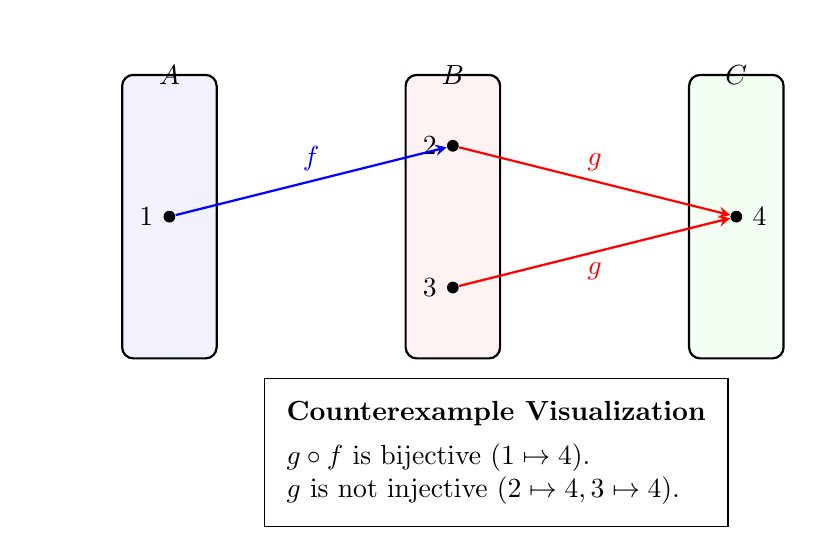
\begin{tikzpicture}[scale=1.2, >=stealth]
    % Background to ensure safe rendering
    \fill[white] (-1,-2) rectangle (7,2);
    
    % Sets
    \draw[thick, rounded corners, fill=blue!5] (0,-1.5) rectangle (1,1.5) node[pos=0.5, yshift=1.8cm] {$A$};
    \draw[thick, rounded corners, fill=red!5] (3,-1.5) rectangle (4,1.5) node[pos=0.5, yshift=1.8cm] {$B$};
    \draw[thick, rounded corners, fill=green!5] (6,-1.5) rectangle (7,1.5) node[pos=0.5, yshift=1.8cm] {$C$};
    
    % Elements
    \node[circle, fill=black, inner sep=1.5pt, label=left:$1$] (a1) at (0.5, 0) {};
    \node[circle, fill=black, inner sep=1.5pt, label=left:$2$] (b1) at (3.5, 0.75) {};
    \node[circle, fill=black, inner sep=1.5pt, label=left:$3$] (b2) at (3.5, -0.75) {};
    \node[circle, fill=black, inner sep=1.5pt, label=right:$4$] (c1) at (6.5, 0) {};
    
    % Arrows
    \draw[->, thick, blue] (a1) -- (b1) node[midway, above] {$f$};
    \draw[->, thick, red] (b1) -- (c1) node[midway, above] {$g$};
    \draw[->, thick, red] (b2) -- (c1) node[midway, below] {$g$};
    
    % Legend
    \node[align=left, draw, fill=white, inner sep=8pt, anchor=west] at (1.5, -2.5) {
        \textbf{Counterexample Visualization} \\[4pt]
        $g \circ f$ is bijective ($1 \mapsto 4$). \\
        $g$ is not injective ($2 \mapsto 4, 3 \mapsto 4$).
    };
\end{tikzpicture}
\end{center}
\vspace{1em}
\end{proof}

\begin{proof}[Solution to Problem 19]
Using the same sets and functions from Problem 18: $A = \{1\}$, $B = \{2, 3\}$, $C = \{4\}$. $f(1) = 2$, $g(2) = 4$, $g(3) = 4$. \\
The composition $g \circ f : A \to C$ is bijective. However, the element $3 \in B$ has no pre-image in $A$ under $f$. Thus, $f$ is not surjective.
\end{proof}

\begin{proof}[Solution to Problem 20]
\textbf{Forward Direction ($\implies$):} Assume $f : A \to B$ is bijective. We construct $g : B \to A$. Let $b \in B$. Because $f$ is surjective, there exists $a \in A$ such that $f(a) = b$. Because $f$ is injective, this $a$ is unique. We define $g(b) = a$. \\
For any $a \in A$, $(g \circ f)(a) = g(f(a))$. Let $f(a) = b$. By our definition of $g$, $g(b) = a$. Thus $(g \circ f)(a) = a$, so $g \circ f = \text{id}_A$. \\
For any $b \in B$, $(f \circ g)(b) = f(g(b))$. Let $g(b) = a$. By definition, $f(a) = b$. Thus $(f \circ g)(b) = b$, so $f \circ g = \text{id}_B$. \\
\textbf{Reverse Direction ($\impliedby$):} Assume there exists $g : B \to A$ such that $g \circ f = \text{id}_A$ and $f \circ g = \text{id}_B$. \\
\textit{Injectivity of $f$:} Let $f(a_1) = f(a_2)$. Applying $g$ to both sides gives $g(f(a_1)) = g(f(a_2)) \implies (g \circ f)(a_1) = (g \circ f)(a_2) \implies \text{id}_A(a_1) = \text{id}_A(a_2) \implies a_1 = a_2$. Thus $f$ is injective. \\
\textit{Surjectivity of $f$:} Let $b \in B$. We need an $a \in A$ such that $f(a) = b$. Let $a = g(b)$. Then $f(a) = f(g(b)) = (f \circ g)(b) = \text{id}_B(b) = b$. Thus $f$ is surjective. \\
Therefore, $f$ is bijective.
\end{proof}

\begin{proof}[Solution to Problem 21]
To be a valid function, every element $a \in A$ must map to exactly one element $b \in B$. Let us test $a = 1 \in A$. \\
We need to find $b \in B = \{2, 4, 6, 8\}$ such that $1 \mid b$ and $b/1$ is odd. \\
- For $b = 2$: $2/1 = 2$ (even). \\
- For $b = 4$: $4/1 = 4$ (even). \\
- For $b = 6$: $6/1 = 6$ (even). \\
- For $b = 8$: $8/1 = 8$ (even). \\
There is no element $b \in B$ that satisfies the relation for $a = 1$. Since the domain element 1 has no output, $R$ is not a function.
\end{proof}

\begin{proof}[Solution to Problem 22]
Since $\Z_5$ is a finite set and the domain and codomain are the same size, by the Pigeonhole Principle, we only need to prove injectivity to establish bijectivity. \\
Let $a, b \in \Z_5$ and assume $f(a) = f(b)$. \\
$3a + 2 \equiv 3b + 2 \pmod 5$ \\
$3a \equiv 3b \pmod 5$ \\
Since $\gcd(3, 5) = 1$, 3 has a multiplicative inverse modulo 5 (which is 2, since $3 \times 2 = 6 \equiv 1 \pmod 5$). Multiplying both sides by 2: \\
$2(3a) \equiv 2(3b) \pmod 5 \implies a \equiv b \pmod 5$. \\
Thus, $f$ is injective. Because $\Z_5$ is finite, $f$ is also surjective, and therefore bijective.
\end{proof}

\begin{proof}[Solution to Problem 23]
We test for injectivity by looking for a counterexample. Notice that $\gcd(2, 6) = 2 \neq 1$, so 2 does not have a multiplicative inverse modulo 6. This suggests it will fail injectivity. \\
Let $x = 0$. $f(0) = 2(0) + 1 = 1 \pmod 6$. \\
Let $x = 3$. $f(3) = 2(3) + 1 = 7 \equiv 1 \pmod 6$. \\
Since $f(0) = f(3)$ but $0 \not\equiv 3 \pmod 6$, the function $f$ is not injective.
\end{proof}

\begin{proof}[Solution to Problem 24]
Let $|A| = |B| = n$. \\
\textbf{Forward ($\implies$):} Assume $f$ is injective. Then $f$ maps the $n$ distinct elements of $A$ to $n$ distinct elements in $B$. Thus, the image $f(A)$ has exactly $n$ elements. Since $f(A) \subseteq B$ and $|B| = n$, it must be that $f(A) = B$. Therefore, $f$ is surjective. \\
\textbf{Reverse ($\impliedby$):} Assume $f$ is surjective. Then $f(A) = B$, meaning the image has $n$ elements. If $f$ were not injective, at least two elements in $A$ would map to the same element in $B$, meaning the image could have at most $n - 1$ elements. This contradicts $|f(A)| = n$. Thus, $f$ must be injective.
\end{proof}

\begin{proof}[Solution to Problem 25]
Let $A = \{a_1, a_2, a_3, a_4, a_5\}$ and $B = \{b_1, b_2, b_3, b_4\}$. A function $f : A \to B$ assigns each of the 5 elements of $A$ to one of the 4 elements of $B$. We can think of the elements of $A$ as "pigeons" and the elements of $B$ as "holes". Since there are 5 pigeons and 4 holes, and $5 > 4$, the Pigeonhole Principle states that at least one hole must contain more than one pigeon. Mathematically, there must exist distinct $a_i, a_j \in A$ such that $f(a_i) = f(a_j)$. Therefore, $f$ cannot be injective.
\end{proof}

\begin{proof}[Solution to Problem 26]
Assume for the sake of contradiction that there exists a surjective function $f : A \to \mathcal{P}(A)$. \\
Consider the set $D = \{ x \in A \mid x \notin f(x) \}$. Since $D$ is a subset of $A$, $D \in \mathcal{P}(A)$. \\
Because $f$ is surjective, there must exist some $d \in A$ such that $f(d) = D$. \\
We now ask: is $d \in D$? \\
Case 1: If $d \in D$, then by the definition of $D$, $d \notin f(d)$. Since $f(d) = D$, this means $d \notin D$, a contradiction. \\
Case 2: If $d \notin D$, then $d \notin f(d)$. By the definition of $D$, this means $d \in D$, a contradiction. \\
Both cases lead to a logical contradiction. Therefore, our assumption that a surjective function $f$ exists must be false.
\end{proof}

\begin{proof}[Solution to Problem 27]
\textbf{Injectivity:} Let $a, b \ge 0$ and assume $F(a) = F(b)$. \\
$1 - e^{-\lambda a} = 1 - e^{-\lambda b} \implies e^{-\lambda a} = e^{-\lambda b}$. \\
Taking the natural logarithm of both sides: $-\lambda a = -\lambda b \implies a = b$. Thus, $F$ is injective. \\
\textbf{Surjectivity:} Let $y \in [0, 1)$. We set $1 - e^{-\lambda x} = y$ and solve for $x$: \\
$e^{-\lambda x} = 1 - y \implies -\lambda x = \ln(1 - y) \implies x = -\frac{1}{\lambda} \ln(1 - y)$. \\
Since $y \in [0, 1)$, $1 - y \in (0, 1]$, so $\ln(1 - y) \le 0$. Since $\lambda > 0$, $x \ge 0$. Thus $x \in [0, \infty)$, so $F$ is surjective. \\
\textbf{Inverse Transform:} To simulate $X$, we set $U = F(X)$ where $U \sim \text{Uniform}(0,1)$. \\
$U = 1 - e^{-\lambda X} \implies e^{-\lambda X} = 1 - U \implies X = -\frac{1}{\lambda} \ln(1 - U)$. \\
(Note: Since $U$ and $1-U$ have the same Uniform(0,1) distribution, this is often simplified in practice to $X = -\frac{1}{\lambda} \ln(U)$).
\end{proof}

\begin{proof}[Solution to Problem 28]
To prove $f(x) = x + \sigma(x)$ is injective on $\R$, we can show it is strictly monotonic by analyzing its first derivative. \\
$f'(x) = 1 + \sigma'(x)$. \\
The derivative of the sigmoid function is $\sigma'(x) = \sigma(x)(1 - \sigma(x))$. \\
Since $0 < \sigma(x) < 1$ for all $x \in \R$, it follows that $0 < \sigma(x)(1 - \sigma(x)) \le 0.25$. \\
Therefore, $f'(x) = 1 + \sigma(x)(1 - \sigma(x)) > 1 > 0$ for all $x \in \R$. \\
Because $f'(x) > 0$ everywhere, $f$ is strictly increasing on $\R$. A strictly increasing function never takes the same value twice, meaning $a < b \implies f(a) < f(b) \implies f(a) \neq f(b)$. Thus, $f$ is injective.
\end{proof}

\begin{proof}[Solution to Problem 29]
\textbf{The Flaw:} The proof assumes that $x = \sqrt{y}$ is a valid real number for \textit{every} $y \in \R$. However, the square root function is only defined over the real numbers for $y \ge 0$. If we choose $y = -1 \in \R$, then $x = \sqrt{-1} \notin \R$. Because there is no real number $x$ such that $x^2 = -1$, the element $-1$ has no pre-image. The function is not surjective, and the proof's algebraic manipulation ignored the domain restrictions of the square root operation.
\end{proof}

\begin{proof}[Solution to Problem 30]
\textbf{The Flaw:} The proof correctly deduces that $g(f(a_1)) = g(f(a_2))$ implies $f(a_1) = f(a_2)$ because $g$ is injective. However, the very next step claims that $f(a_1) = f(a_2) \implies a_1 = a_2$. This deduction is only valid if the inner function $f$ is injective. The problem statement did not assume $f$ is injective. Therefore, the proof makes an unjustified logical leap. (In fact, the theorem itself is false; $g \circ f$ being injective requires $f$ to be injective, not $g$).
\end{proof}

\newpage

\section{Concept Checklist \& Question Mapping (Repeated)}

\renewcommand{\arraystretch}{1.5}
\begin{tabularx}{\textwidth}{l X >{$\displaystyle}c<{$}}
\toprule
\textbf{ID} & \textbf{Concept / Technique} & \text{\textbf{Mapped Problems}} \\
\midrule
C1 & Algebraic Verification of Injectivity (Direct Proof) & 1, 2, 3, 5, 28 \\
C2 & Algebraic Verification of Surjectivity (Direct Proof) & 1, 3, 4, 5, 27 \\
C3 & Counterexample Generation (Falsifying Injectivity) & 4, 6, 7, 9, 10, 23 \\
C4 & Counterexample Generation (Falsifying Surjectivity) & 2, 6, 7, 8, 10 \\
C5 & Abstract Set-Theoretic Proofs (Element-Chasing) & 11, 12, 13, 14, 15 \\
C6 & Function Composition Properties ($g \circ f$) & 16, 17, 18, 19, 20 \\
C7 & Pigeonhole Principle \& Cardinality Arguments & 8, 9, 24, 25, 26 \\
C8 & Relations vs. Functions (Well-definedness) & 21 \\
C9 & Modular Arithmetic in Relations \& Functions & 22, 23 \\
C10 & Real-World Modeling (CDFs, Inverse Transform, ML) & 27, 28 \\
C11 & Identifying Logical Flaws in Proofs & 29, 30 \\
\bottomrule
\end{tabularx}

\end{document}